\documentclass[a4paper, 12pt]{article}%тип документа

\usepackage{placeins}
%отступы
\usepackage[left=2cm,right=2cm,top=2cm,bottom=3cm,bindingoffset=0cm]{geometry}

%Русский язык
\usepackage[T2A]{fontenc} %кодировка
\usepackage[utf8]{inputenc} %кодировка исходного кода
\usepackage[english,russian]{babel} %локализация и переносы

%Вставка картинок
\usepackage{wrapfig}
\usepackage{graphicx}
\graphicspath{{pictures/}}
\DeclareGraphicsExtensions{.pdf,.png,.jpg}

%Графики
\usepackage{multirow}
\usepackage{pgfplots}
\pgfplotsset{compat=1.9}

%Математика
\usepackage{amsmath, amsfonts, amssymb, amsthm, mathtools}

%Заголовок
\author{Мыздриков Иван Витальевич\\
Б06-401}
\title{\textbf{Работа 2.2.3 \\ 
Измерение теплопроводности воздуха при атмосферном давлении}}
\begin{document}
\maketitle
\newpage
\section*{Теоретическая справка}
\textit{Теплопроводность} — это процесс передачи тепловой энергии от нагретых частей системы к холодным за счёт хаотического движения частиц среды (молекул, атомов и т.п.). В газах теплопроводность осуществляется за счёт  непосредственной передачи кинетической энергии от быстрых молекул к медленным при их столкновениях. Перенос тепла описывается законом Фурье, утверждающим, что плотность потока энергии 
\newline
$\overline{q} = -k \nabla T$, где $k \left[ \dfrac{\text{Вт}}{\text{м} \cdot \text{К}} \right]$ - \textit{коэффициент теплопроводности}.

Молекулярно-кинетическая теория дает следующую оценку для коэффициента теплопроводности газов: 
\[k \sim \lambda \overline{\nu} \cdot n c_V \text{.}\]
С помощью некоторых преобразований мы получаем, что 
\[ Q = \dfrac{2 \pi L}{\ln \dfrac{r_0}{r_1}} k  \cdot \Delta T \text{.}\]
\section*{Экспериментальная установка}
\begin{wrapfigure}{r}{0.4\textwidth}
  \begin{center}
    \includegraphics[width = 0.3\textwidth]{7.png}
  \end{center}
  \textbf{\caption{Схема установки}}
\end{wrapfigure}
Схема установки приведена на рис. 1. На оси полой цилиндрической трубки с внутренним диаметром $2r_0 \sim 0.7$ см размещена металлическая нить диаметром $2r_1 \sim 0,05$ мм и длиной $L \sim 40$ см (материал нити и точные геометрические размеры указаны в техническом описании установки). Полость трубки заполнена воздухом (полость через небольшое отверстие сообщается с атмосферой). Стенки трубки помещены в кожух, через которых пропускается вода из термостата, так что их температура $t_0$ поддерживается постоянной. Для предотвращения конвекции трубка расположена вертикально.

Металлическая нить служит как источником тепла, так и датчиком температуры (термометром сопротивления). По пропускаемому через нить постоянному току $I$ и напряжению $U$ на ней вычисляется мощность нагрева по закону Джоуля–Ленца: $Q = UI$, и сопротивление нити по закону Ома: $R = \dfrac{U}{I}$.

Сопротивление нити является однозначной функцией её температуры $R (t)$.
Эта зависимость может быть измерена с помощью термостата по экстраполяции мощности нагрева к нулю $Q \rightarrow 0$, когда температура нити и стенок совпадают $t_1 \approx t_0$. Альтернативно, если материал нити известен, зависимость его удельного сопротивления от температуры может найдена по справочным данным.
\newpage
На рис. 2 представлена схема электрической установки:
\begin{wrapfigure}{r}{0.6\textwidth}
  \begin{center}
    \includegraphics[width = 0.5\textwidth]{8.png}
  \end{center}
  \textbf{\caption{Электрическая схема измерения сопротивления нити и мощности нагрева}}
\end{wrapfigure}
Схема рис. 2 предусматривает использование одного вольтметра и одного амперметра, магазина сопротивлений $R_{\text{м}}$, включённого последовательно с источником напряжения и нитью.
\section*{Методика измерений} 
Принципиально неустранимая систематическая ошибка измерения температуры с помощью термометра сопротивления возникает из-за необходимости пропускать через резистор (нить) измерительный ток. Чем этот ток выше, тем с большей точностью будет измерен как он сам, так и напряжение. Однако при этом квадратично возрастает выделяющаяся на  резисторе мощность $Q = UI = I^2R$. Следовательно, температура резистора становится выше, чем у объекта, температуру которого надо измерить. Измерения же при малых токах не дают достаточной точности (в частности, из-за существенного вклада термоэлектрических явлений в проводниках и контактах). Эта проблема решается построением нагрузочной кривой - зависимости измеряемого сопротивления $R$ от выделяющейся в нём мощности $R(Q)$, с последующей экстраполяцией к нулевой мощности $Q \to 0$ для определения сопротивления $R_0 = R(0)$, при котором его температура равна температуре измеряемого объекта. Кроме того, в данной работе измерение нагрузочных кривых позволяет в ходе эксперимента получить температурную зависимость сопротивления нити, так как при $Q \to 0$ температура нити равна температуре термостата ($T \approx T_0$). В исследуемом интервале температур (20-80 $^0C$) зависимость сопротивления от температуры можно с хорошей точностью аппроксимировать линейной функцией:
\[R(t) = R_{273} \cdot (1 + \alpha t)\]
где $\alpha = \dfrac{1}{R_{273}} \dfrac{dR}{dT}$ - температурный коэффициент сопротивления материала.
\section*{Ход работы}
\begin{enumerate}
\item При комнатной температуре термостата измеряем зависимость сопротивления нити $R =\dfrac{U}{I}$ от подаваемой на неё мощности $Q = UI$ - нагрузочную кривую $R(Q)$.

Измерения проводим для 7-9 различных значений силы тока через нить от 0 до $I_{max}$.
\begin{table}[h]
\begin{center}
\begin{tabular}{|c|c|c|c|}
\hline
\multicolumn{4}{|c|}{$T = 23 ^0 C$} \\ \hline
$Q,$ Дж & $\varepsilon_Q,$ Дж & $R$, Ом & $\varepsilon_R$, Ом \\ \hline
0.003 & 0.0005 & 19.593 & 0.0005 \\ \hline
0.011 & 0.0005 & 19.625 & 0.0005 \\ \hline
0.024 & 0.0005 & 20.205 & 0.0005 \\ \hline
0.04 & 0.0005 & 19.911 & 0.0005 \\ \hline
0.06 & 0.0005 & 20.073 & 0.0005 \\ \hline
0.083 & 0.0005 & 20.0 & 0.0005 \\ \hline
0.123 & 0.0005 & 18.083 & 0.0005 \\ \hline
0.172 & 0.0005 & 20.939 & 0.0005 \\ \hline
0.202 & 0.0005 & 20.833 & 0.0005 \\ \hline
\end{tabular}
\end{center}
\caption{Данные для комнатной температуры}
\end{table} 
\item Проводим измерения нагрузочных кривых согласно п. 1 для 5–7 температур термостата в диапазоне от комнатной до 80 $^0 C$.
\begin{table}[h]
\begin{center}
\begin{tabular}{|c|c|c|c|}
\hline
\multicolumn{4}{|c|}{$T = 32 ^0 C$} \\ \hline
$Q,$ Дж & $\varepsilon_Q,$ Дж & $R$, Ом & $\varepsilon_R$, Ом \\ \hline
0.003 & 0.0005 & 21.61 & 0.0005 \\ \hline
0.011 & 0.0005 & 19.888 & 0.0005 \\ \hline
0.023 & 0.0005 & 20.103 & 0.0005 \\ \hline
0.04 & 0.0005 & 20.196 & 0.0005 \\ \hline
0.06 & 0.0005 & 20.312 & 0.0005 \\ \hline
0.102 & 0.0005 & 19.867 & 0.0005 \\ \hline
0.11 & 0.0005 & 20.606 & 0.0005 \\ \hline
0.138 & 0.0005 & 20.751 & 0.0005 \\ \hline
0.168 & 0.0005 & 20.922 & 0.0005 \\ \hline
0.199 & 0.0005 & 21.092 & 0.0005 \\ \hline
\end{tabular}
\end{center}
\caption{Данные для $T = 32 ^0 C$}
\end{table}
\FloatBarrier
\begin{table}[h]
\begin{center}
\begin{tabular}{|c|c|c|c|}
\hline
\multicolumn{4}{|c|}{$T = 44.3 ^0 C$} \\ \hline
$Q,$ Дж & $\varepsilon_Q,$ Дж & $R$, Ом & $\varepsilon_R$, Ом \\ \hline
0.003 & 0.0005 & 21.084 & 0.0005 \\ \hline
0.011 & 0.0005 & 21.131 & 0.0005 \\ \hline
0.024 & 0.0005 & 21.199 & 0.0005 \\ \hline
0.041 & 0.0005 & 21.288 & 0.0005 \\ \hline
0.061 & 0.0005 & 21.397 & 0.0005 \\ \hline
0.085 & 0.0005 & 21.521 & 0.0005 \\ \hline
0.11 & 0.0005 & 21.656 & 0.0005 \\ \hline
0.138 & 0.0005 & 21.798 & 0.0005 \\ \hline
0.168 & 0.0005 & 21.953 & 0.0005 \\ \hline
0.198 & 0.0005 & 22.107 & 0.0005 \\ \hline
\end{tabular}
\end{center}
\caption{Данные для $T = 44.3 ^0 C$}
\end{table}
\FloatBarrier
\FloatBarrier
\begin{table}[h]
\begin{center}
\begin{tabular}{|c|c|c|c|}
\hline
\multicolumn{4}{|c|}{$T = 55 ^0 C$} \\ \hline
$Q,$ Дж & $\varepsilon_Q,$ Дж & $R$, Ом & $\varepsilon_R$, Ом \\ \hline
0.003 & 0.0005 & 21.842 & 0.0005 \\ \hline
0.011 & 0.0005 & 21.883 & 0.0005 \\ \hline
0.025 & 0.0005 & 21.952 & 0.0005 \\ \hline
0.042 & 0.0005 & 22.04 & 0.0005 \\ \hline
0.092 & 0.0005 & 32.676 & 0.0005 \\ \hline
0.085 & 0.0005 & 22.263 & 0.0005 \\ \hline
0.111 & 0.0005 & 22.39 & 0.0005 \\ \hline
0.138 & 0.0005 & 22.527 & 0.0005 \\ \hline
0.167 & 0.0005 & 22.673 & 0.0005 \\ \hline
0.197 & 0.0005 & 22.818 & 0.0005 \\ \hline
\end{tabular}
\end{center}
\caption{Данные для $T = 55 ^0 C$}
\end{table}
\FloatBarrier
\FloatBarrier
\begin{table}[h]
\begin{center}
\begin{tabular}{|c|c|c|c|}
\hline
\multicolumn{4}{|c|}{$T = 78 ^0 C$} \\ \hline
$Q,$ Дж & $\varepsilon_Q,$ Дж & $R$, Ом & $\varepsilon_R$, Ом \\ \hline
0.005 & 0.0005 & 16.274 & 0.0005 \\ \hline
0.012 & 0.0005 & 23.288 & 0.0005 \\ \hline
0.025 & 0.0005 & 23.354 & 0.0005 \\ \hline
0.043 & 0.0005 & 23.441 & 0.0005 \\ \hline
0.063 & 0.0005 & 23.543 & 0.0005 \\ \hline
0.086 & 0.0005 & 23.651 & 0.0005 \\ \hline
0.112 & 0.0005 & 23.772 & 0.0005 \\ \hline
0.138 & 0.0005 & 23.899 & 0.0005 \\ \hline
0.167 & 0.0005 & 23.857 & 0.0005 \\ \hline
0.194 & 0.0005 & 24.162 & 0.0005 \\ \hline
\end{tabular}
\end{center}
\caption{Данные для $T = 78 ^0 C$}
\end{table}
\FloatBarrier

\FloatBarrier
\begin{figure}[h]
\center{\includegraphics[width = 0.9\textwidth]{1.jpg}}
\caption{График для $T = 23 ^0 C$}
\end{figure}
\FloatBarrier
\FloatBarrier
\begin{figure}[h]
\center{\includegraphics[width = 0.9\textwidth]{2.jpg}}
\caption{График для $T = 32 ^0 C$}
\end{figure}
\FloatBarrier
\FloatBarrier
\begin{figure}[h]
\center{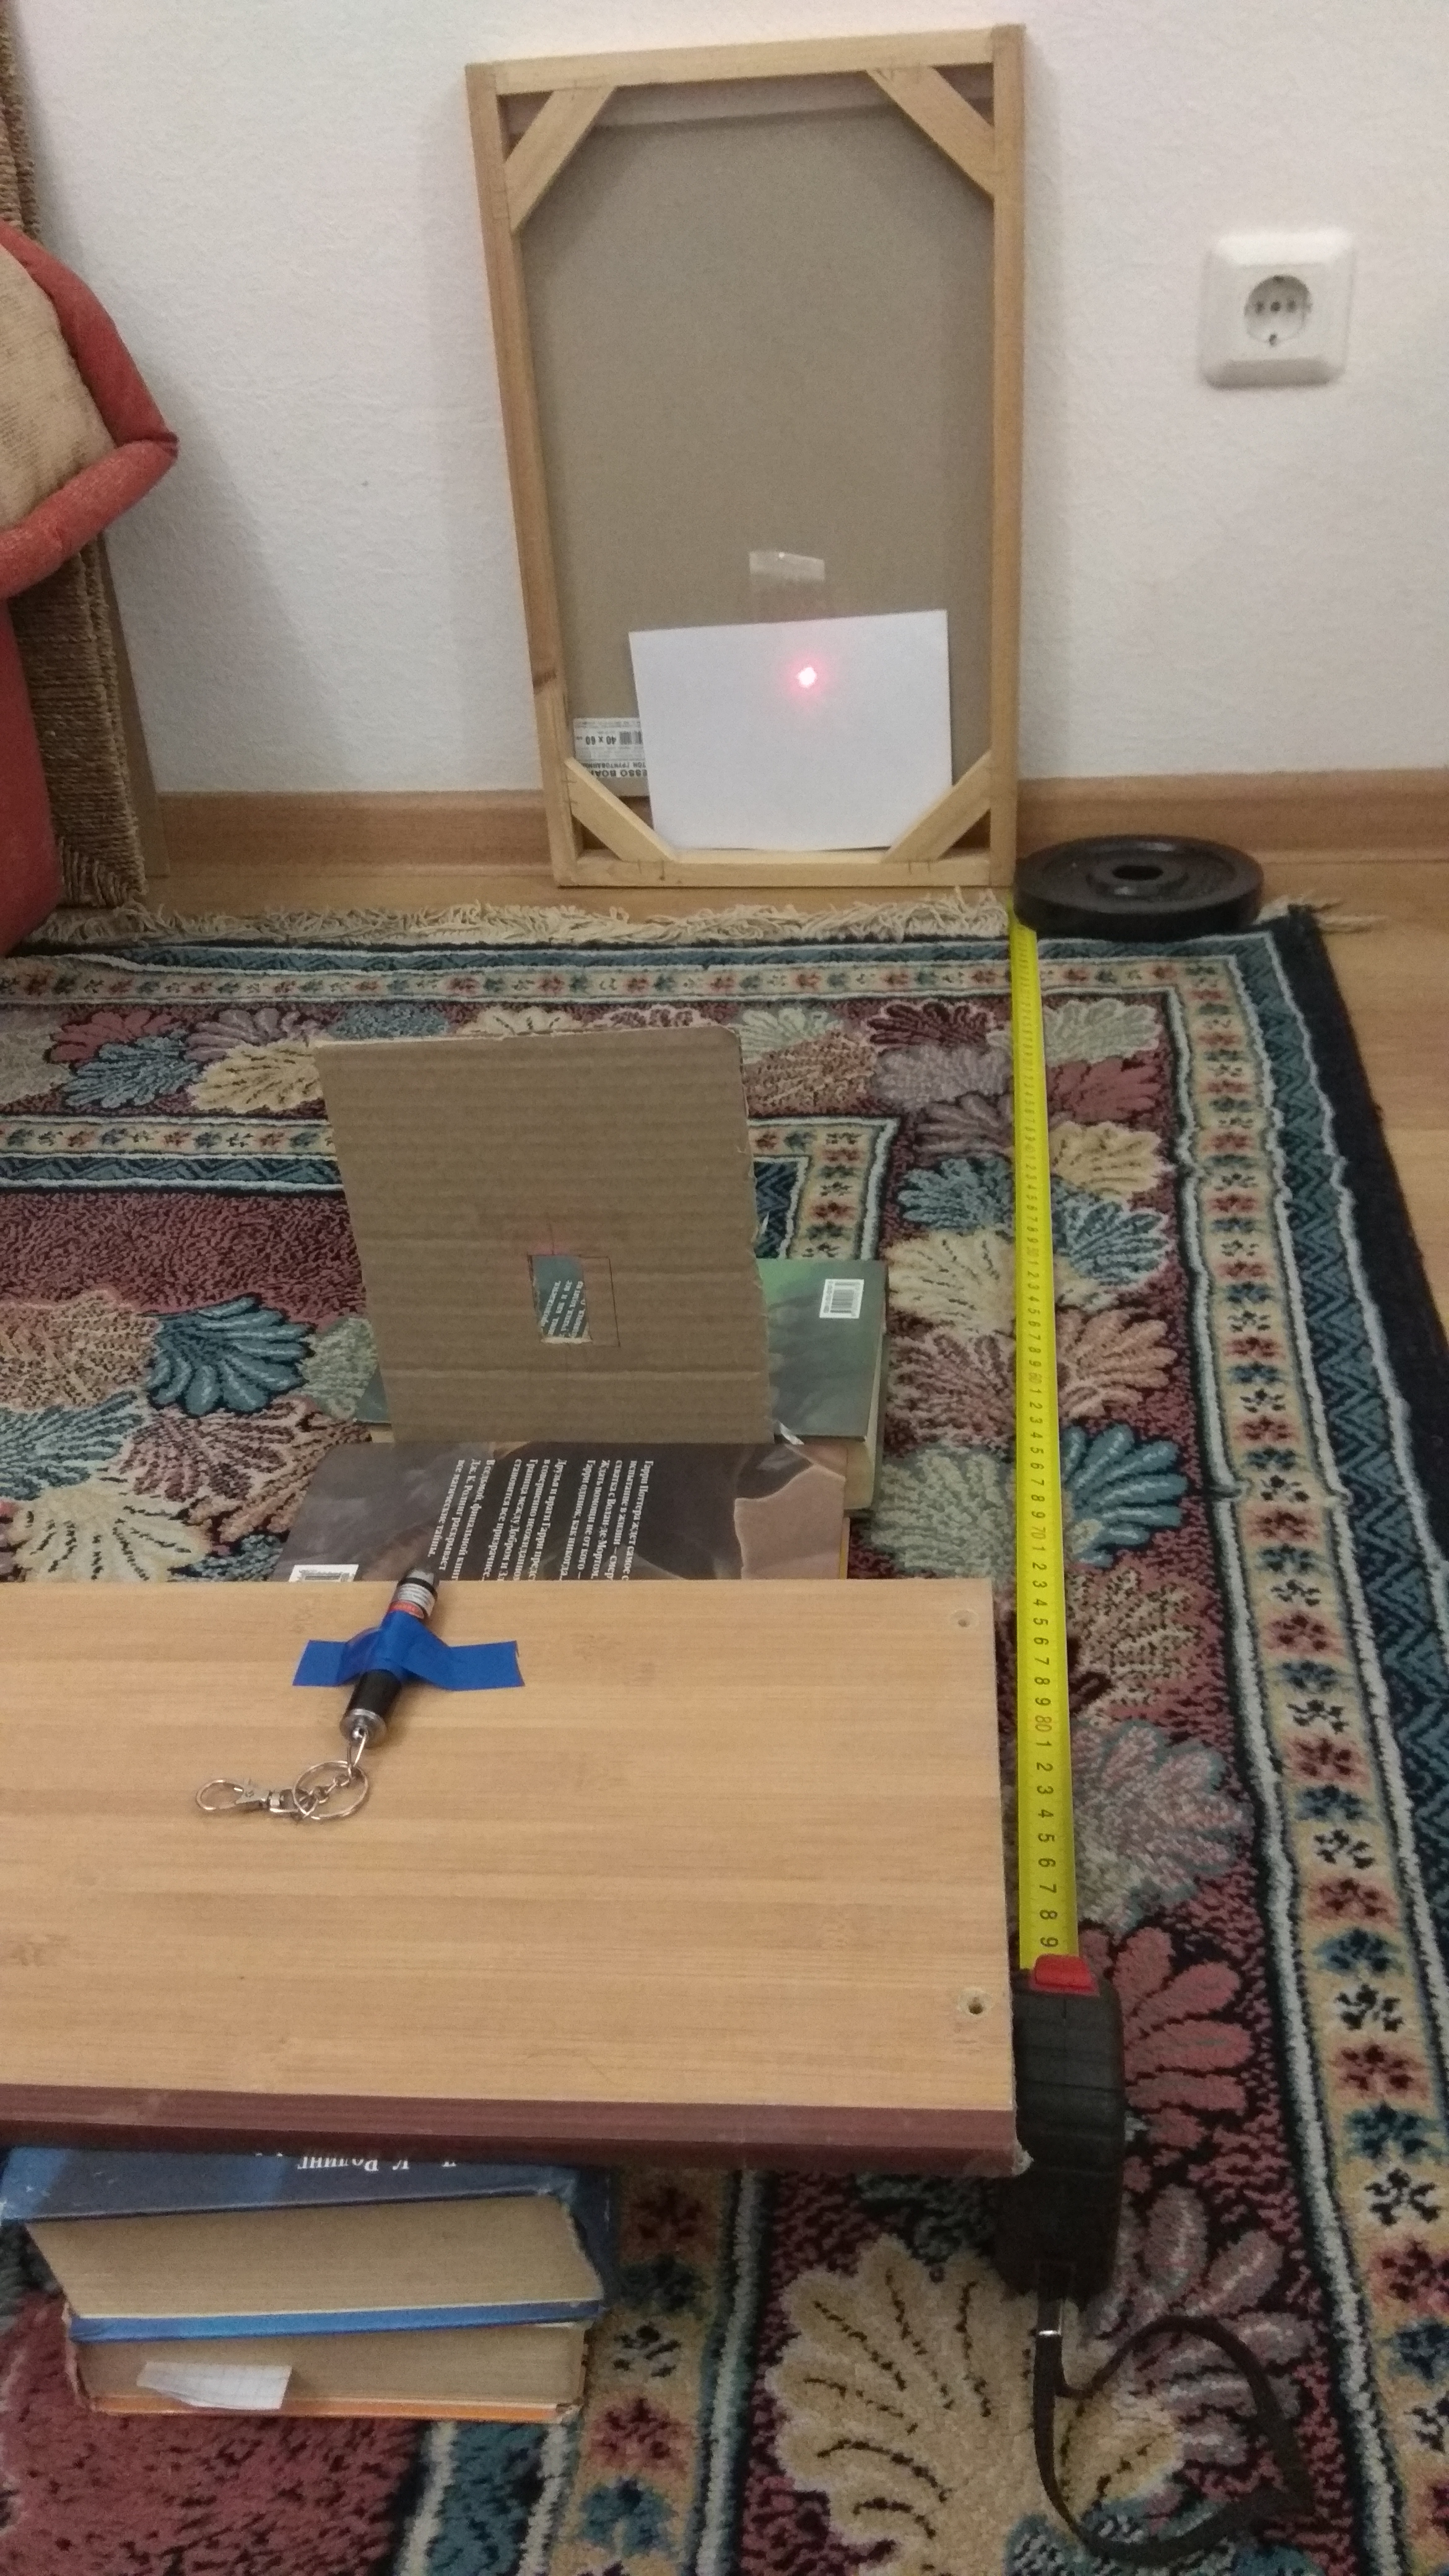
\includegraphics[width = 0.9\textwidth]{3.jpg}}
\caption{График для $T = 44.3 ^0 C$}
\end{figure}
\FloatBarrier
\FloatBarrier
\begin{figure}[h]
\center{\includegraphics[width = 0.9\textwidth]{4.jpg}}
\caption{График для $T = 55 ^0 C$}
\end{figure}
\FloatBarrier
\FloatBarrier
\begin{figure}[h]
\center{\includegraphics[width = 0.9\textwidth]{5.jpg}}
\caption{График для $T = 78 ^0 C$}
\end{figure}
\FloatBarrier
\FloatBarrier
\item теперь обработаем результаты, запишем все наклоны и $R_0$ из графиков в одну таблицу
\begin{table}[h]
\begin{tabular}{|c|c|c|c|c|}
\hline
$T$, K & $dR/dQ$, Ом/Дж & $\sigma_{dR/dQ}$,  Ом/Дж & $R_0$, Ом & $\sigma_{R_0}$, Ом \\ \hline
296 & 6.2 & 0,8 & 19.7 & 0,03 \\ \hline
305 & 6.0 & 0,8 & 19.9 & 0,2 \\ \hline
317.3 & 5.2 & 0,07 & 21 & 0,002 \\ \hline
328 & 5.1 & 1,3 & 21.8 & 0,01 \\ \hline
351 & 4,4  & 1 & 23.2 & 0,1 \\ \hline
\end{tabular}
\end{table}
\FloatBarrier
\begin{figure}[h]
\center{\includegraphics[width = 0.9\textwidth]{9.jpg}}
\caption{График $R(T)$}
\end{figure}
\FloatBarrier
\begin{table}[h]
\begin{tabular}{|c|c|c|c|c|c|c|}
\hline
$T$, K & $dR/dQ$, Ом/Дж & $R_0$, Ом & $\sigma_{R_0}$, Ом & $(dR/dT)/(dR/dQ)$, Дж/К & $k$, Вт/м К & $\sigma_k$, Вт/м К \\ \hline
296   & 6.2 & 19.7 & 0,03 & 0,0665 & 0,131 & 0,002 \\ \hline
305   & 6.0 & 19.9  & 0,2 & 0,0652 & 0,128 & 0,002 \\ \hline
317.3 & 5.2 & 21 & 0,002  & 0,0662 & 0,130 & 0,002 \\ \hline
328   & 5.1 & 21.8 & 0,01 & 0,0665 & 0,131 & 0,002 \\ \hline
351   & 4.4 & 23.2  & 0,1 & 0,0661 & 0,129 & 0,002 \\ \hline
\end{tabular}
\caption{Таблица $k$}
\end{table}
\end{enumerate}
\end{document}